\documentclass{article}

\usepackage[english]{babel}
\usepackage[utf8]{inputenc}
\usepackage{amsmath}
\usepackage{amsthm}
\usepackage{amssymb}
\usepackage{mathtools}
\usepackage{amsfonts}
\usepackage{subcaption}
\usepackage{graphicx}
\usepackage{wrapfig}
\usepackage{bbm}
\usepackage{dsfont}
\usepackage{listings}

% set up margin
\usepackage
[
  a4paper,
  left=3cm,
  right=3cm,
  top=3cm,
  bottom=3cm,
]
{geometry}

% set up header
\usepackage{fancyhdr}
\pagestyle{fancy}
\fancyhf{}
\lhead{6.438 Algorithms for Inference}
\chead{Problem Set 6}
\rhead{Hongzi Mao}
\cfoot{\thepage}
\rfoot{\footnotesize{\emph{Collaborated with: Hongzhou Ye, Zhiwei Ding}}}

% footer line
\renewcommand{\footrulewidth}{0.4pt}

% sans serif italic
\newcommand{\s}[1]{\textsf{\textit{#1}}}

% bold face sans serif
\newcommand{\bs}[1]{\textsf{\textbf{#1}}}

% set symbol
\usepackage[mathscr]{euscript}

% empty set
\let\emptyset\varnothing

% qed
\newcommand{\qeds}{\hfill\qedsymbol}

% math bold face
\newcommand{\bm}{\mathbf}

% argmax
\DeclareMathOperator*{\argmax}{argmax}
\DeclareMathOperator*{\argmin}{argmin}

% colorful reference
\usepackage{hyperref}
\usepackage{color}
\definecolor{darkred}{rgb}{0.7,0,0}
\definecolor{darkgreen}{rgb}{0,0.5,0}
\hypersetup{colorlinks=true,
        linkcolor=darkred,
        citecolor=darkgreen}
\urlstyle{same}

% independence symbol
\makeatletter
\newcommand*{\indep}{%
  \mathbin{%
    \mathpalette{\@indep}{}%
  }%
}
\newcommand*{\nindep}{%
  \mathbin{%                   % The final symbol is a binary math operator
    \mathpalette{\@indep}{\not}% \mathpalette helps for the adaptation
                               % of the symbol to the different math styles.
  }%
}
\newcommand*{\@indep}[2]{%
  \sbox0{$#1\perp\m@th$}%        box 0 contains \perp symbol
  \sbox2{$#1=$}%                 box 2 for the height of =
  \sbox4{$#1\vcenter{}$}%        box 4 for the height of the math axis
  \rlap{\copy0}%                 first \perp
  \dimen@=\dimexpr\ht2-\ht4-.2pt\relax
  \kern\dimen@
  {#2}
  \kern\dimen@
  \copy0 %                       second \perp
} 
\makeatother

%%%%%%%%%%%%%%%%%%%%%%%%%%%%%%%%%%%%%%%%%%%%%%%%%%%%%%%%%%%%%%%%%%%%%%%%
%%%%%%%%%%%%%%%%%%%%%%%%% Begin document here %%%%%%%%%%%%%%%%%%%%%%%%%%
%%%%%%%%%%%%%%%%%%%%%%%%%%%%%%%%%%%%%%%%%%%%%%%%%%%%%%%%%%%%%%%%%%%%%%%%
\begin{document}
\section*{Problem 6.3}
%
\textbf{Key routines in the program.}
\\

%
\noindent
For Gibbs node-by-node sampler, the key routines are 
\begin{enumerate}
	\item Initialization of node values (e.g., all $+1$ or all $-1$). Initialization of edge potentials. (Figure~\ref{f:code}a)
	\item In each iteration on a node, compute the probability of choosing $+1$, based on edge potential
	  	  and the values of the neighbor nodes. The probability is computed
	  	  in Equation~(1) from Problem 6.2. (Figure~\ref{f:code}b)
	\item A loop through all nodes in each sampling iteration. (Figure~\ref{f:code}c)
\end{enumerate}
%
For Gibbs comb block sampler, the key routines are
\begin{enumerate}
	\item Initialization of node values (e.g., all $+1$ or all $-1$). Initialization of edge potentials. This
	      step is the same as Gibbs node-by-node sampler. (Figure~\ref{f:code}a)
	\item A message update routine to aggregate messages for specified destination (requiring source message all aggregated). 
	      (Figure~\ref{f:code}d)
	\item A serial belief propagation routine that calls the message update following a traversal order
	      (from the proper indexing in Problem 6.2(b)). (Figure~\ref{f:code}e)
	\item A scheme to determine the tree traversal order (indexing) for the two combs. (Figure~\ref{f:code}f)
	\item In each iteration on a node, update the node and edge potential in the tree path, and then
	      perform serial belief propagation to get all the messages on one direction.
	      Start sampling from the marginals. Based on the sampled value and passed messages,
	      sample the conditional probability using Equation~(2) from Problem 6.2(b). (Figure~\ref{f:code}g)
	\item A loop through all nodes in each sampling iteration. (Figure~\ref{f:code}h)\\
\end{enumerate}

\noindent
\textbf{Visualization of the samples.}
\\

\noindent
We run the Gibbs node-by-node sampler for 1000 iterations, initializing from all $+1$ or all $-1$ for the nodes.
The samples are visualized every 100 steps. The samples from initialization $+1$ is in Figure~\ref{f:63a}.
The samples from initialization $-1$ is in Figure~\ref{f:63b}.
\\
%

\noindent
Similarly, we run the Gibbs block sampler for 1000 iterations, also initializing from all $+1$ or all $-1$ for the nodes.
The samples from initialization $+1$ is in Figure~\ref{f:63c}.
The samples from initialization $-1$ is in Figure~\ref{f:63d}.
%
\begin{figure*}[h]
\captionsetup[subfigure]{labelformat=empty}
\centering
\begin{subfigure}[t]{0.18\textwidth}
\centering
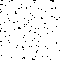
\includegraphics[width=\textwidth]{./computational/results/gibbs_node_sampler_positive_iter_0.png}
\vspace{-0.6cm}
\caption{iteration=1}
\end{subfigure}\hspace{0.01\textwidth}
\begin{subfigure}[t]{0.18\textwidth}
\centering

\includegraphics[width=\textwidth]{./computational/results/gibbs_node_sampler_positive_iter_100.png}
\vspace{-0.6cm}
\caption{iteration=100}
\end{subfigure}\hspace{0.01\textwidth}
\begin{subfigure}[t]{0.18\textwidth}
\centering

\includegraphics[width=\textwidth]{./computational/results/gibbs_node_sampler_positive_iter_200.png}
\vspace{-0.6cm}
\caption{iteration=200}
\end{subfigure}\hspace{0.01\textwidth}
\begin{subfigure}[t]{0.18\textwidth}
\centering

\includegraphics[width=\textwidth]{./computational/results/gibbs_node_sampler_positive_iter_300.png}
\vspace{-0.6cm}
\caption{iteration=300}
\end{subfigure}\hspace{0.01\textwidth}
\begin{subfigure}[t]{0.18\textwidth}
\centering

\includegraphics[width=\textwidth]{./computational/results/gibbs_node_sampler_positive_iter_400.png}
\vspace{-0.6cm}
\caption{iteration=400}
\end{subfigure}\hspace{0.01\textwidth}
\begin{subfigure}[t]{0.18\textwidth}
\centering

\includegraphics[width=\textwidth]{./computational/results/gibbs_node_sampler_positive_iter_500.png}
\vspace{-0.6cm}
\caption{iteration=500}
\end{subfigure}\hspace{0.01\textwidth}
\begin{subfigure}[t]{0.18\textwidth}
\centering

\includegraphics[width=\textwidth]{./computational/results/gibbs_node_sampler_positive_iter_600.png}
\vspace{-0.6cm}
\caption{iteration=600}
\end{subfigure}\hspace{0.01\textwidth}
\begin{subfigure}[t]{0.18\textwidth}
\centering

\includegraphics[width=\textwidth]{./computational/results/gibbs_node_sampler_positive_iter_700.png}
\vspace{-0.6cm}
\caption{iteration=700}
\end{subfigure}\hspace{0.01\textwidth}
\begin{subfigure}[t]{0.18\textwidth}
\centering

\includegraphics[width=\textwidth]{./computational/results/gibbs_node_sampler_positive_iter_800.png}
\vspace{-0.6cm}
\caption{iteration=800}
\end{subfigure}\hspace{0.01\textwidth}
\begin{subfigure}[t]{0.18\textwidth}
\centering

\includegraphics[width=\textwidth]{./computational/results/gibbs_node_sampler_positive_iter_900.png}
\vspace{-0.6cm}
\caption{iteration=900}
\end{subfigure}\hspace{0.01\textwidth}
\caption{Visualizing the node-by-node Gibbs sampling results. $+1$ is indicated by white in the image. The values are initialized as $+1$.}
\label{f:63a}
\end{figure*}
%
\begin{figure*}[h]
\captionsetup[subfigure]{labelformat=empty}
\centering
\begin{subfigure}[t]{0.18\textwidth}
\centering

\includegraphics[width=\textwidth]{./computational/results/gibbs_node_sampler_negative_iter_0.png}
\vspace{-0.6cm}
\caption{iteration=1}
\end{subfigure}\hspace{0.01\textwidth}
\begin{subfigure}[t]{0.18\textwidth}
\centering

\includegraphics[width=\textwidth]{./computational/results/gibbs_node_sampler_negative_iter_100.png}
\vspace{-0.6cm}
\caption{iteration=100}
\end{subfigure}\hspace{0.01\textwidth}
\begin{subfigure}[t]{0.18\textwidth}
\centering

\includegraphics[width=\textwidth]{./computational/results/gibbs_node_sampler_negative_iter_200.png}
\vspace{-0.6cm}
\caption{iteration=200}
\end{subfigure}\hspace{0.01\textwidth}
\begin{subfigure}[t]{0.18\textwidth}
\centering

\includegraphics[width=\textwidth]{./computational/results/gibbs_node_sampler_negative_iter_300.png}
\vspace{-0.6cm}
\caption{iteration=300}
\end{subfigure}\hspace{0.01\textwidth}
\begin{subfigure}[t]{0.18\textwidth}
\centering

\includegraphics[width=\textwidth]{./computational/results/gibbs_node_sampler_negative_iter_400.png}
\vspace{-0.6cm}
\caption{iteration=400}
\end{subfigure}\hspace{0.01\textwidth}
\begin{subfigure}[t]{0.18\textwidth}
\centering

\includegraphics[width=\textwidth]{./computational/results/gibbs_node_sampler_negative_iter_500.png}
\vspace{-0.6cm}
\caption{iteration=500}
\end{subfigure}\hspace{0.01\textwidth}
\begin{subfigure}[t]{0.18\textwidth}
\centering

\includegraphics[width=\textwidth]{./computational/results/gibbs_node_sampler_negative_iter_600.png}
\vspace{-0.6cm}
\caption{iteration=600}
\end{subfigure}\hspace{0.01\textwidth}
\begin{subfigure}[t]{0.18\textwidth}
\centering

\includegraphics[width=\textwidth]{./computational/results/gibbs_node_sampler_negative_iter_700.png}
\vspace{-0.6cm}
\caption{iteration=700}
\end{subfigure}\hspace{0.01\textwidth}
\begin{subfigure}[t]{0.18\textwidth}
\centering

\includegraphics[width=\textwidth]{./computational/results/gibbs_node_sampler_negative_iter_800.png}
\vspace{-0.6cm}
\caption{iteration=800}
\end{subfigure}\hspace{0.01\textwidth}
\begin{subfigure}[t]{0.18\textwidth}
\centering

\includegraphics[width=\textwidth]{./computational/results/gibbs_node_sampler_negative_iter_900.png}
\vspace{-0.6cm}
\caption{iteration=900}
\end{subfigure}\hspace{0.01\textwidth}
\caption{Visualizing the node-by-node Gibbs sampling results. $+1$ is indicated by white in the image. The values are initialized as $-1$.}
\label{f:63b}
\end{figure*}
%
\pagebreak
%
\begin{figure*}[h]
\captionsetup[subfigure]{labelformat=empty}
\centering
\begin{subfigure}[t]{0.18\textwidth}
\centering
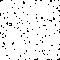
\includegraphics[width=\textwidth]{./computational/results/gibbs_comb_sampler_positive_iter_0.png}
\vspace{-0.6cm}
\caption{iteration=1}
\end{subfigure}\hspace{0.01\textwidth}
\begin{subfigure}[t]{0.18\textwidth}
\centering

\includegraphics[width=\textwidth]{./computational/results/gibbs_comb_sampler_positive_iter_100.png}
\vspace{-0.6cm}
\caption{iteration=100}
\end{subfigure}\hspace{0.01\textwidth}
\begin{subfigure}[t]{0.18\textwidth}
\centering

\includegraphics[width=\textwidth]{./computational/results/gibbs_comb_sampler_positive_iter_200.png}
\vspace{-0.6cm}
\caption{iteration=200}
\end{subfigure}\hspace{0.01\textwidth}
\begin{subfigure}[t]{0.18\textwidth}
\centering

\includegraphics[width=\textwidth]{./computational/results/gibbs_comb_sampler_positive_iter_300.png}
\vspace{-0.6cm}
\caption{iteration=300}
\end{subfigure}\hspace{0.01\textwidth}
\begin{subfigure}[t]{0.18\textwidth}
\centering

\includegraphics[width=\textwidth]{./computational/results/gibbs_comb_sampler_positive_iter_400.png}
\vspace{-0.6cm}
\caption{iteration=400}
\end{subfigure}\hspace{0.01\textwidth}
\begin{subfigure}[t]{0.18\textwidth}
\centering
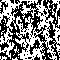
\includegraphics[width=\textwidth]{./computational/results/gibbs_comb_sampler_positive_iter_500.png}
\vspace{-0.6cm}
\caption{iteration=500}
\end{subfigure}\hspace{0.01\textwidth}
\begin{subfigure}[t]{0.18\textwidth}
\centering
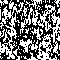
\includegraphics[width=\textwidth]{./computational/results/gibbs_comb_sampler_positive_iter_600.png}
\vspace{-0.6cm}
\caption{iteration=600}
\end{subfigure}\hspace{0.01\textwidth}
\begin{subfigure}[t]{0.18\textwidth}
\centering
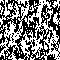
\includegraphics[width=\textwidth]{./computational/results/gibbs_comb_sampler_positive_iter_700.png}
\vspace{-0.6cm}
\caption{iteration=700}
\end{subfigure}\hspace{0.01\textwidth}
\begin{subfigure}[t]{0.18\textwidth}
\centering
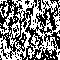
\includegraphics[width=\textwidth]{./computational/results/gibbs_comb_sampler_positive_iter_800.png}
\vspace{-0.6cm}
\caption{iteration=800}
\end{subfigure}\hspace{0.01\textwidth}
\begin{subfigure}[t]{0.18\textwidth}
\centering

\includegraphics[width=\textwidth]{./computational/results/gibbs_comb_sampler_positive_iter_900.png}
\vspace{-0.6cm}
\caption{iteration=900}
\end{subfigure}\hspace{0.01\textwidth}
\caption{Visualizing the comb block Gibbs sampling results. $+1$ is indicated by white in the image. The values are initialized as $+1$.}
\label{f:63c}
\end{figure*}
%
\begin{figure*}[h]
\captionsetup[subfigure]{labelformat=empty}
\centering
\begin{subfigure}[t]{0.18\textwidth}
\centering

\includegraphics[width=\textwidth]{./computational/results/gibbs_comb_sampler_negative_iter_0.png}
\vspace{-0.6cm}
\caption{iteration=1}
\end{subfigure}\hspace{0.01\textwidth}
\begin{subfigure}[t]{0.18\textwidth}
\centering

\includegraphics[width=\textwidth]{./computational/results/gibbs_comb_sampler_negative_iter_100.png}
\vspace{-0.6cm}
\caption{iteration=100}
\end{subfigure}\hspace{0.01\textwidth}
\begin{subfigure}[t]{0.18\textwidth}
\centering

\includegraphics[width=\textwidth]{./computational/results/gibbs_comb_sampler_negative_iter_200.png}
\vspace{-0.6cm}
\caption{iteration=200}
\end{subfigure}\hspace{0.01\textwidth}
\begin{subfigure}[t]{0.18\textwidth}
\centering

\includegraphics[width=\textwidth]{./computational/results/gibbs_comb_sampler_negative_iter_300.png}
\vspace{-0.6cm}
\caption{iteration=300}
\end{subfigure}\hspace{0.01\textwidth}
\begin{subfigure}[t]{0.18\textwidth}
\centering

\includegraphics[width=\textwidth]{./computational/results/gibbs_comb_sampler_negative_iter_400.png}
\vspace{-0.6cm}
\caption{iteration=400}
\end{subfigure}\hspace{0.01\textwidth}
\begin{subfigure}[t]{0.18\textwidth}
\centering
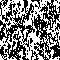
\includegraphics[width=\textwidth]{./computational/results/gibbs_comb_sampler_negative_iter_500.png}
\vspace{-0.6cm}
\caption{iteration=500}
\end{subfigure}\hspace{0.01\textwidth}
\begin{subfigure}[t]{0.18\textwidth}
\centering

\includegraphics[width=\textwidth]{./computational/results/gibbs_comb_sampler_negative_iter_600.png}
\vspace{-0.6cm}
\caption{iteration=600}
\end{subfigure}\hspace{0.01\textwidth}
\begin{subfigure}[t]{0.18\textwidth}
\centering

\includegraphics[width=\textwidth]{./computational/results/gibbs_comb_sampler_negative_iter_700.png}
\vspace{-0.6cm}
\caption{iteration=700}
\end{subfigure}\hspace{0.01\textwidth}
\begin{subfigure}[t]{0.18\textwidth}
\centering

\includegraphics[width=\textwidth]{./computational/results/gibbs_comb_sampler_negative_iter_800.png}
\vspace{-0.6cm}
\caption{iteration=800}
\end{subfigure}\hspace{0.01\textwidth}
\begin{subfigure}[t]{0.18\textwidth}
\centering

\includegraphics[width=\textwidth]{./computational/results/gibbs_comb_sampler_negative_iter_900.png}
\vspace{-0.6cm}
\caption{iteration=900}
\end{subfigure}\hspace{0.01\textwidth}
\caption{Visualizing the comb block Gibbs sampling results. $+1$ is indicated by white in the image. The values are initialized as $-1$.}
\label{f:63d}
\end{figure*}
%
\\

\noindent
\textbf{Analysis.}
\\

\noindent
By symmetry, there should not be a bias between $+1$ or $-1$ samples.
%
Thus, over a long time, the samples should give $+1$ or $-1$ with the same probability for all nodes.
%
Visually from the samples, the Gibbs block sampler mixes faster.
%
We also plot a time series of average value of all nodes over the evolution steps in Figure~\ref{f:63e}.
%
Clearly, Gibbs block sampler converges to the average value 0 much faster.
%
Running the node-by-node sampler for longer time (Figure~\ref{f:63f}) does yield unbiased samples.
%
But the time scale at least $50\times$ longer (notice the difference in the number of steps).
%

In terms of per-sweep running time, the complexity is both $O(n)$. Since the block sampling scheme has
an extra step for message passing and updating the node potentials from the observation of the other block,
the empirical runtime for the block sampler is slightly longer ($\sim 2\times$ longer in my implementation).

The initialization affects the node-by-node sampler since the mixing behavior is not as fast as the block sampler.
\\

\begin{figure*}[h]
\centering
%
\begin{subfigure}[t]{0.48\textwidth}
\centering
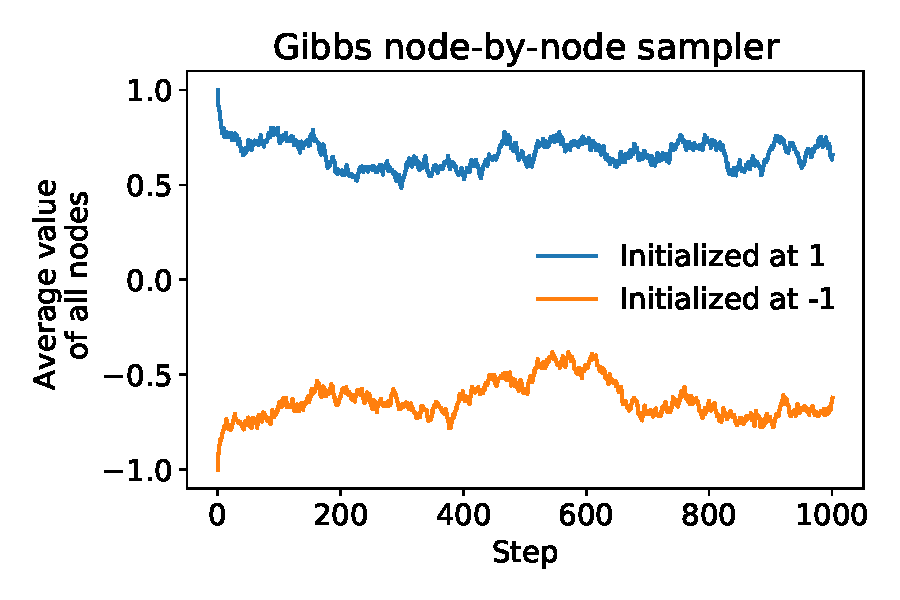
\includegraphics[width=\textwidth]{./computational/gibbs_node_sampler_mixing.pdf}
\vspace{-0.6cm}
\caption{Gibbs node-by-node sampler mixing behavior.}
\end{subfigure}
%
\begin{subfigure}[t]{0.48\textwidth}
\centering
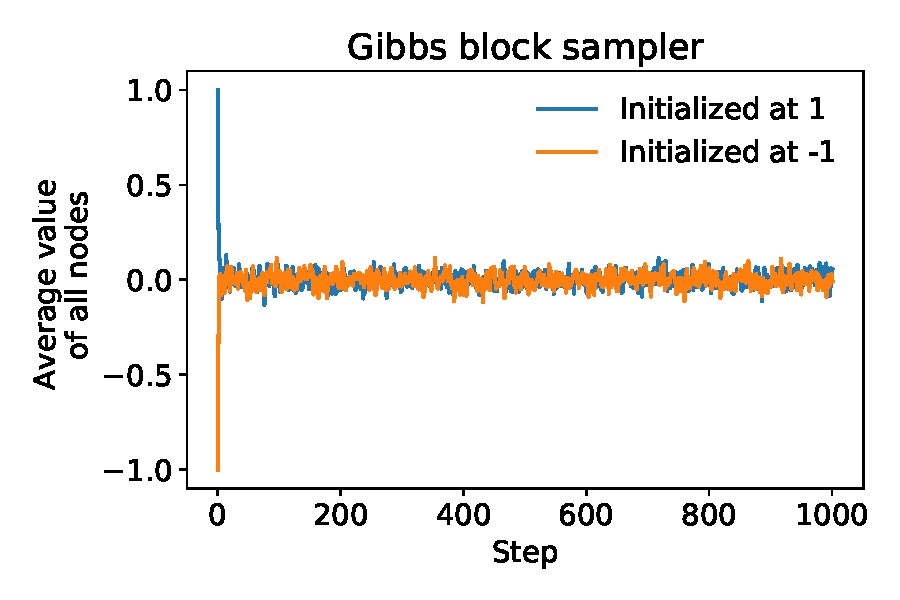
\includegraphics[width=\textwidth]{./computational/gibbs_block_sampler_mixing.pdf}
\vspace{-0.6cm}
\caption{Gibbs comb block sampler mixing behavior.}
\end{subfigure}
%
\caption{Mixing behavior of Gibbs samplers.}
\label{f:63e}
\end{figure*}

\begin{figure*}[h]
\centering
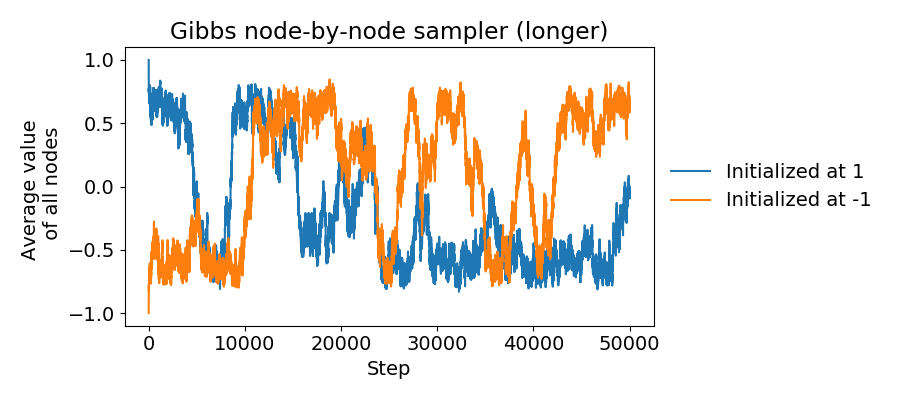
\includegraphics[width=0.8\textwidth]{./computational/gibbs_node_sampler_mixing_longer.png}
\vspace{-0.6cm}
\caption{Mixing behavior of Gibbs node-by-node samplers after running for a longer time.}
\label{f:63f}
\end{figure*}

\noindent
\textbf{Code snippets.}
The code snippets are included in Figure~\ref{f:code}.
%

\begin{figure*}[h]
\centering
\captionsetup[subfigure]{labelformat=empty}
\begin{subfigure}[t]{0.3\textwidth}
\centering
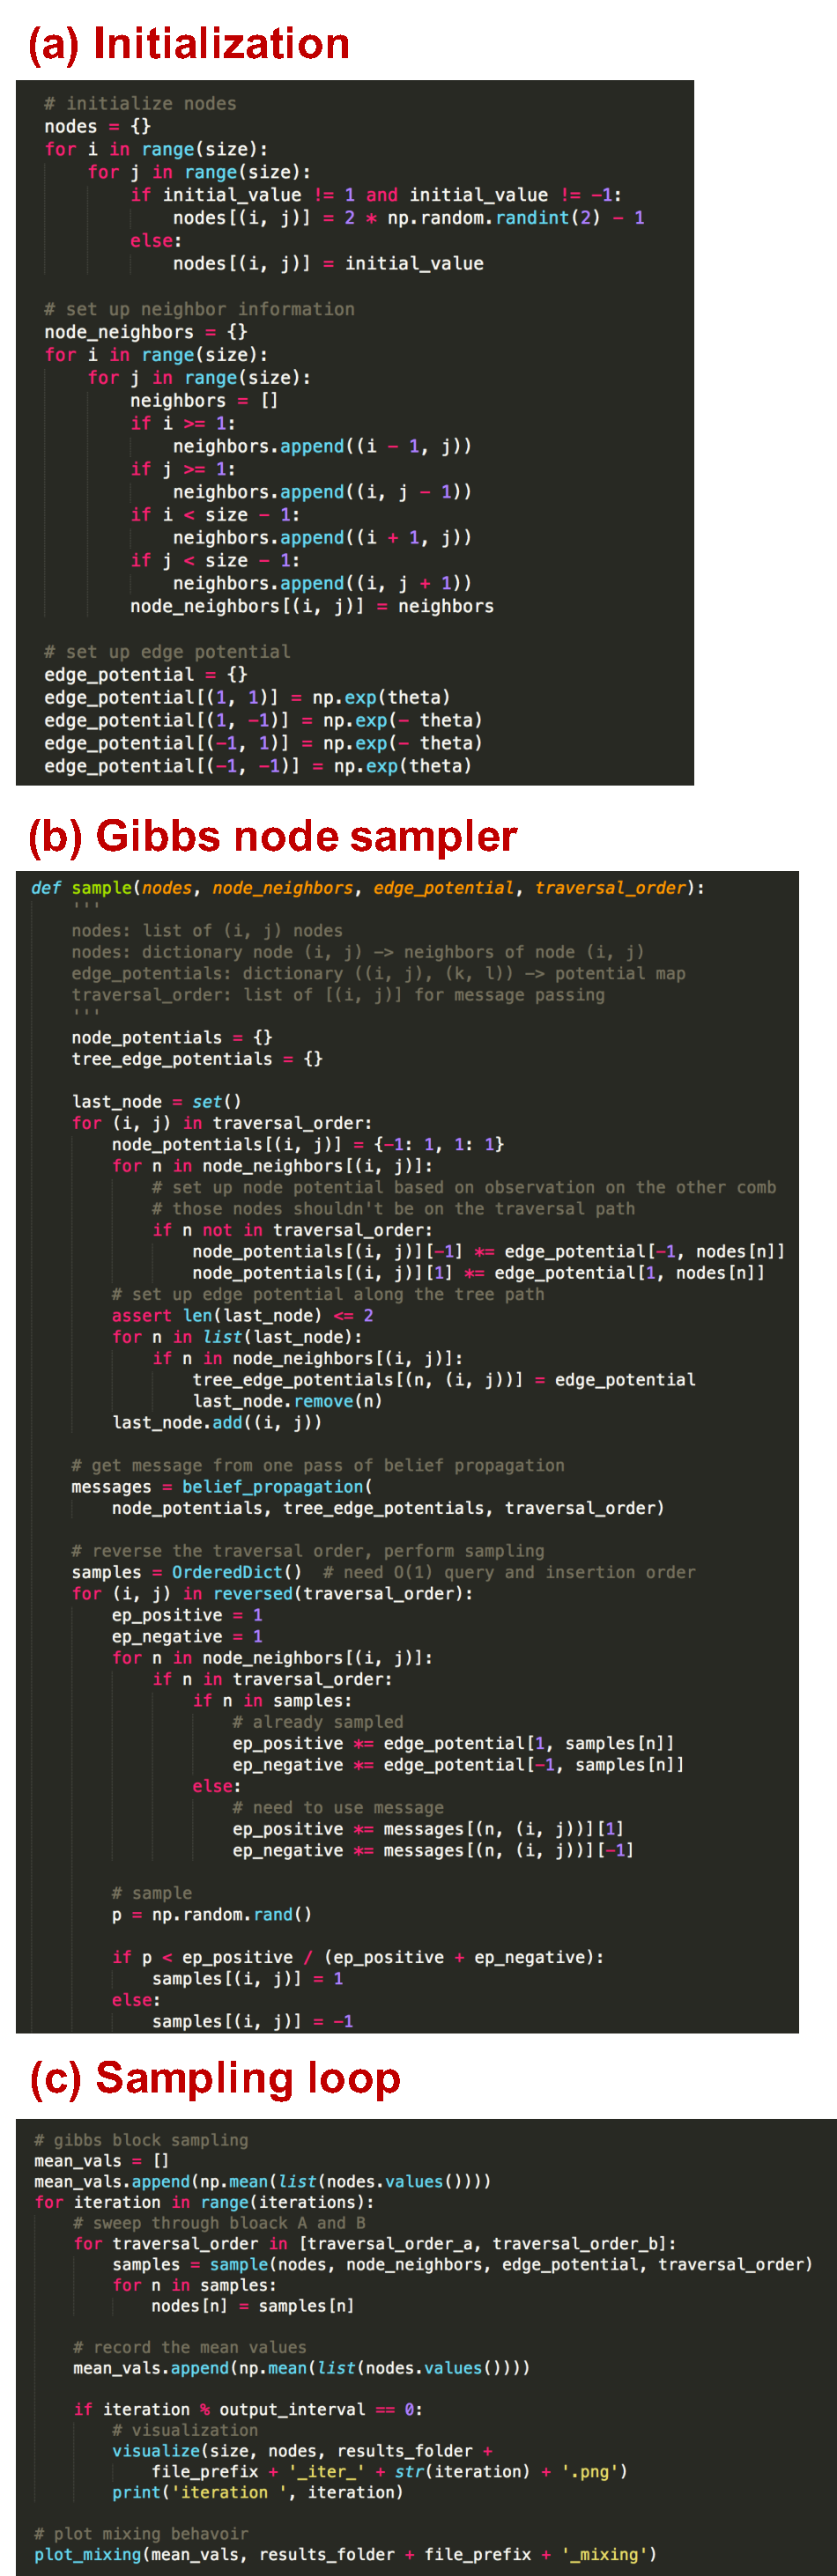
\includegraphics[width=\textwidth]{./computational/code_screenshots/code_1.pdf}
\vspace{-0.6cm}
\label{f:code_node}
\caption{node-by-node.}
\end{subfigure} \hspace{0.02\textwidth}
%
\begin{subfigure}[t]{0.65\textwidth}
\centering
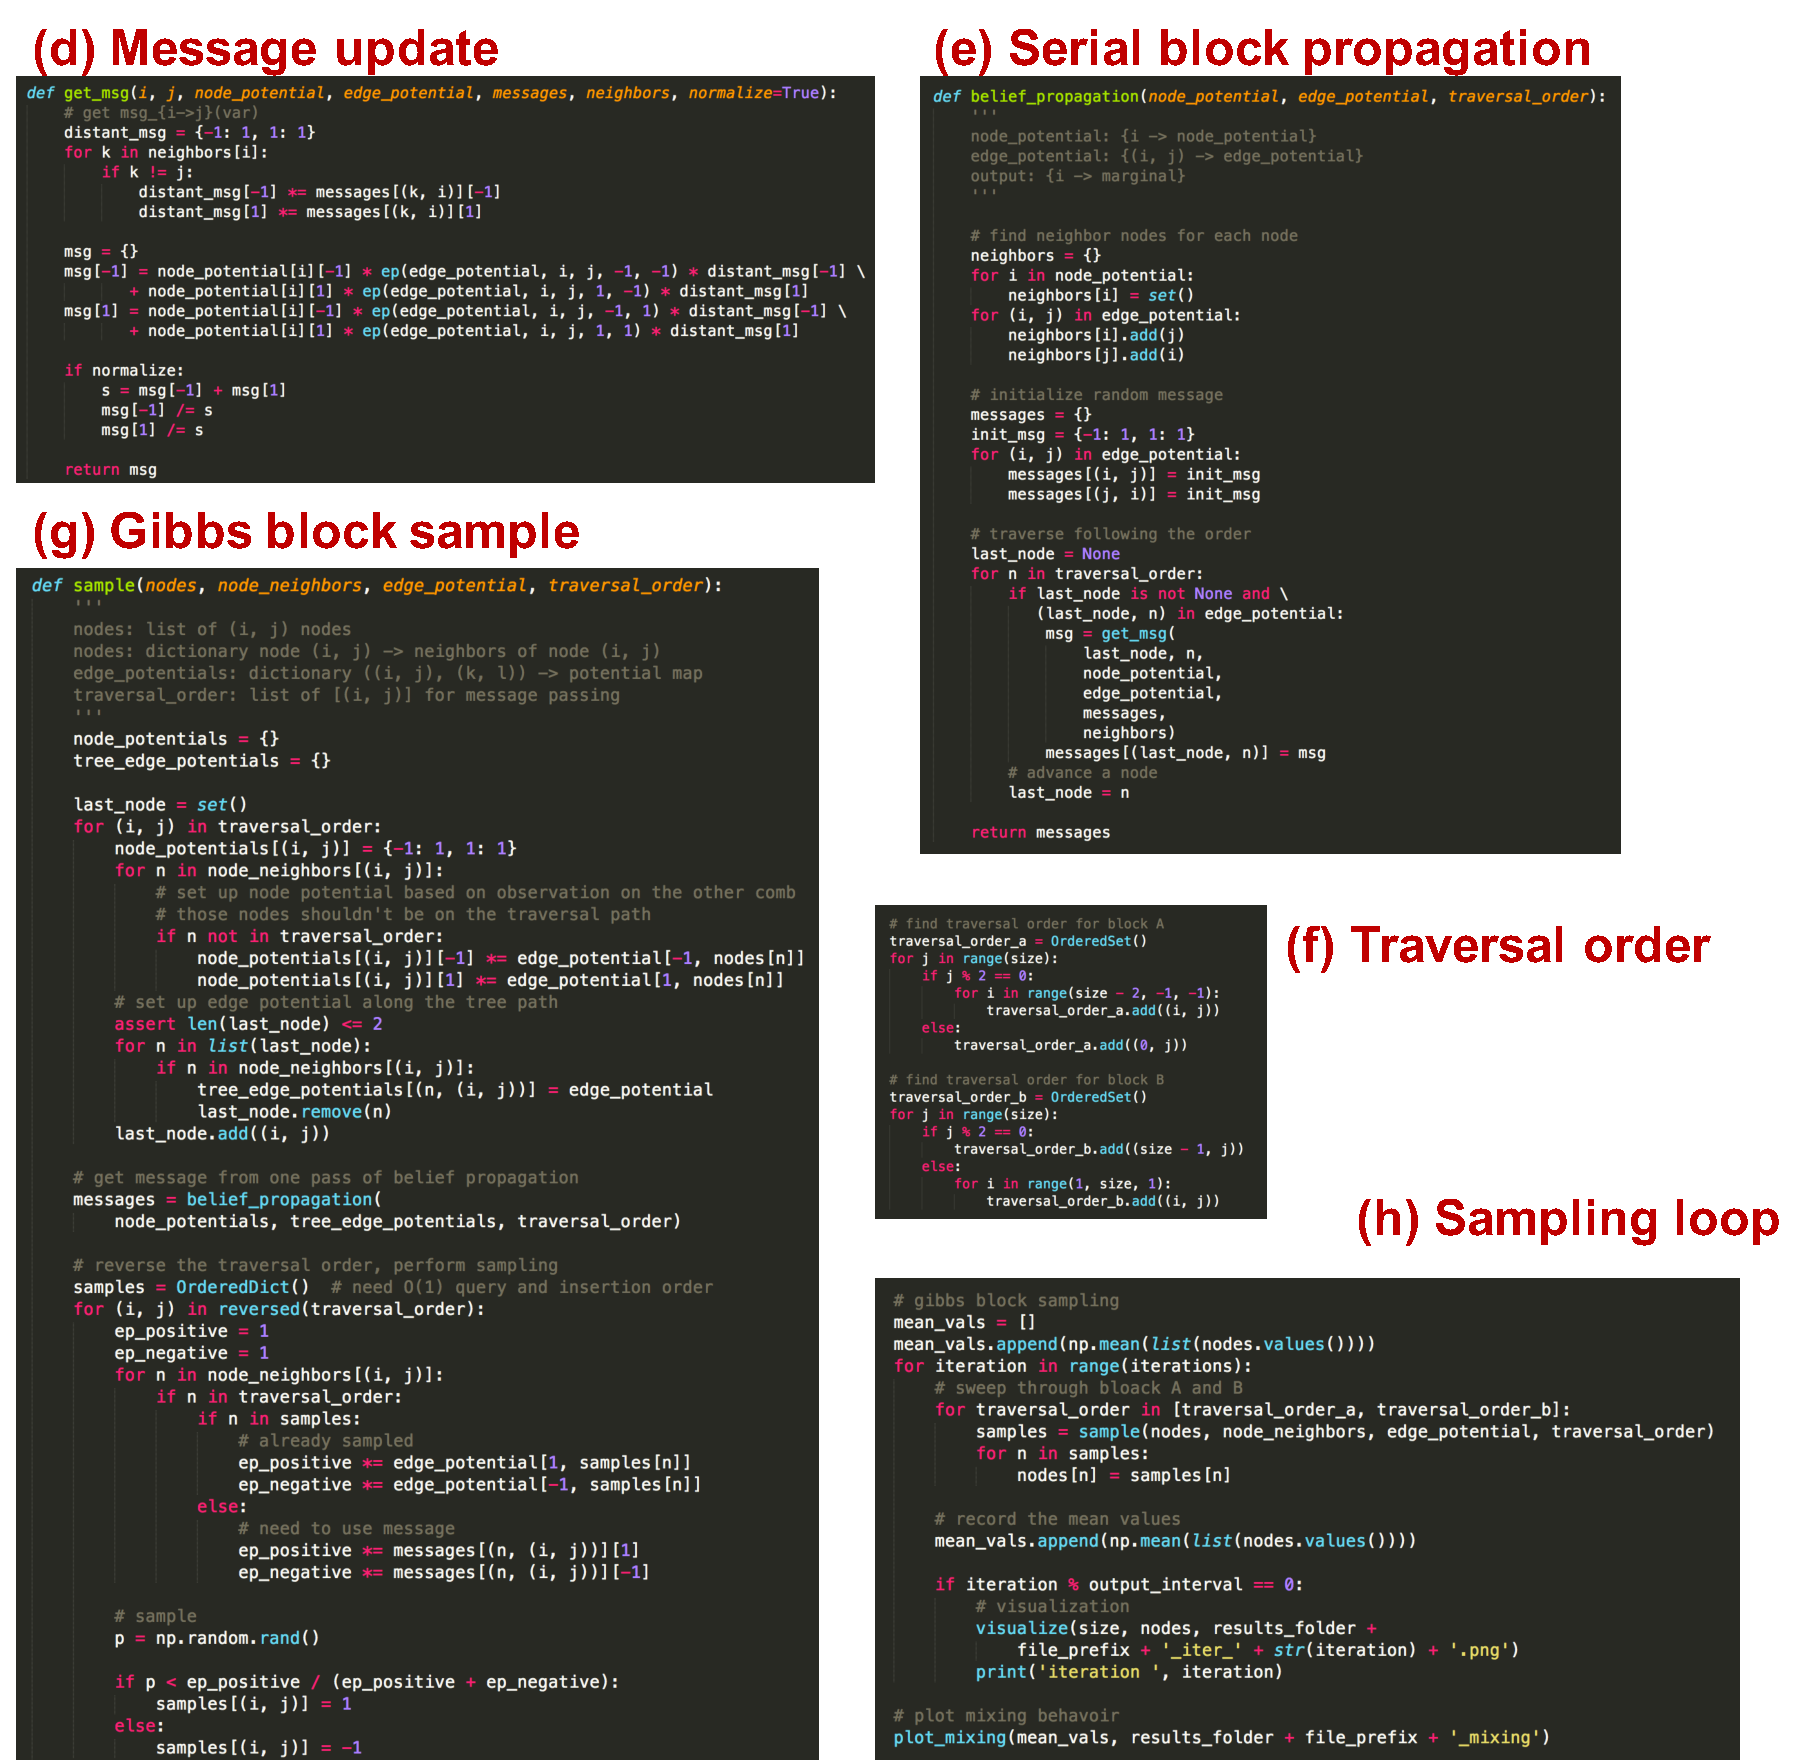
\includegraphics[width=\textwidth]{./computational/code_screenshots/code_2.pdf}
\vspace{-0.6cm}
\label{f:code_block}
\caption{Comb-shaped block.}
\end{subfigure}
%
\caption{Code snippets for Gibbs sampler.}
\label{f:code}
\end{figure*}

\pagebreak

\end{document}